\documentclass[fleqn]{article}
\usepackage[english]{babel}
\usepackage{amsmath}
\usepackage{amsthm}
\usepackage{graphicx}
\usepackage[utf8]{inputenc}

%%%%%%%% MARGIN
\usepackage[left=1in, right=1in, top=0.8in, bottom=0.8in]{geometry}

%%%%%%%% NO PARAGRAPH INDENT
% https://tex.stackexchange.com/questions/27802/set-noindent-for-entire-file
\setlength\parindent{0pt}

%%%%%%%% SUB-FIGURE PACKAGE
\usepackage{subcaption}

\usepackage{pdfpages}

%%%%%%%% HYPERREF PACKAGE
\usepackage{hyperref}
\hypersetup{linkcolor=blue}
\hypersetup{citecolor=blue}
\hypersetup{urlcolor=blue}
\hypersetup{colorlinks=true}

%%%%%%%% MULTI-COLUMNS PACKAGE
\usepackage{multicol}

%%%%%%%% SETS DEFINITIONS
\usepackage{amssymb}
%%%% Important sets
\renewcommand{\O}{\mathbb{O}}
\newcommand{\N}{\mathbb{N}}
\newcommand{\Z}{{\mathbb{Z}}}
\newcommand{\Q}{{\mathbb{Q}}}
\newcommand{\RR}{{\mathbb{R}}}

%%%% Statistics
\newcommand{\E}[1]{\mathbb{E}\left[#1 \right]}
\newcommand{\V}[1]{\mathbb{V}\left[#1 \right]}
\newcommand{\cov}[1]{\mathrm{Cov}\left[#1 \right]}

%%% Misc Math
% Spaces after/before left/right
\let\originalleft\left
\let\originalright\right
\renewcommand{\left}{\mathopen{}\mathclose\bgroup\originalleft}
\renewcommand{\right}{\aftergroup\egroup\originalright}

% Norm and abs
\newcommand{\norm}[1]{\left\lVert#1\right\rVert}
\newcommand{\abs}[1]{\left\lvert#1\right\rvert}

%%%% Superscript to the left
% https://latex.org/forum/viewtopic.php?t=455
\usepackage{tensor}
\newcommand{\app}[3]{\tensor*[^{#1}]{\left(#2, #3\right)}{}}


%%%%%%%% SPLIT EQUATIONS
% https://tex.stackexchange.com/questions/51682/is-it-possible-to-pagebreak-aligned-equations
\allowdisplaybreaks

%%%%%%%% CODE RENDERING
% Compile with flag -shell-escape
\usepackage{minted}

%%%%%%%% EXAM PACKAGE
\usepackage{mathexam}

%%%%%%%% CHANGE MARGINS ITEMIZE
\usepackage{enumitem}

%%%%%%%% START DOCUMENT

\ExamClass{EC0301 - Time Series}
\ExamName{Assignment \#3}
\ExamHead{\today}

\let\ds\displaystyle

\begin{document}
 \vspace{0.3cm}
   % Information of the student
   \begin{itemize}[leftmargin=6.25cm, labelsep=0.5cm]

     \item[\textit{Name}] \scalebox{1.2}{David Plazas Escudero} % Name
     \item[\textit{Student code}] 201710005101 % Code

   \end{itemize}
\vspace{0.3cm}

% Each of the items to solve
\begin{enumerate}
\item \textit{Show the maximum values that $|\rho_1|$ and $|\rho_2|$ can reach on a MA(2) model.}

For this exercise we used a numerical optimization approach, rather than deducing the result theoretically. The problems to solve are formally given as 
\begin{equation}
\begin{split}
\mathrm{max} \ J=\abs{\rho_i(\theta_1, \theta_2)}\\
\text{s.t. } \theta_1,\theta_2\in\RR
\end{split}
\end{equation}
for $i=1,2$, which are unconstrained global optimization problems in the variables $\theta_1$ and $\theta_2$, and where $\rho_i$ is the autocorrelation functions studied in class, namely,
\begin{equation}
    \rho_1(\theta_1, \theta_2) = \dfrac{-\theta_1+\theta_1\theta_2}{1+\theta^2_1+\theta_2^2},\quad \text{and}\quad \rho_2(\theta_1, \theta_2) = \dfrac{-\theta_2}{1+\theta^2_1+\theta_2^2}.
\end{equation}
Given the nature of this optimization problem, it can be easily solved numerically with a gradient descent method. The method will be briefly described:
\begin{itemize}
    \item Define $\theta^k:=\left[\theta_1^k,\theta_2^k\right]^T$ as the value of $\theta_1$ and $\theta_2$ at the iteration $k$. Define $J^k$ in the same manner.
    \item Select $\theta^0\in\RR^2$, $\eta\ll 1$ and $\gamma\lll 1$ as input parameters for the algorithm.
    \item Update $\theta^{k+1}=\theta^{k}+\eta\nabla\rho_i(\theta^k)$.
    \item Check if the condition $\abs{J^{k+1}-J^k}<\gamma$ is met. In that case, return $\theta^{k+1}$, otherwise, set $k=k+1$ and return to the previous step.
\end{itemize}
Let us present the code:
\begin{minted}{python}
import numpy as np
import matplotlib.pyplot as plt

def grad_p1(t):
    t1 = t[0,0]
    t2 = t[1,0]
    term = (1 + t1**2 + t2**2)
    p1 = ((-1 + t2)*term - 2*t1*(-t1 + t1*t2))/(term**2)
    p2 = (t1*term - 2*t2*(-t1 + t1*t2))/(term**2)
    return np.vstack((p1, p2))

def grad_p2(t):
    t1 = t[0,0]
    t2 = t[1,0]
    term = (1 + t1**2 + t2**2)
    p1 = (2*t1*t2)/(term**2)
    p2 = (2*t2**2 - term)/(term**2)
    return np.vstack((p1, p2))

def p1(t):
    t1 = t[0,0]
    t2 = t[1,0]
    return np.abs((-t1 + t1*t2)/(1 + t1**2 + t2**2))


def p2(t):
    t1 = t[0,0]
    t2 = t[1,0]
    return np.abs((-t2)/(1 + t1**2 + t2**2))
    
def optimize(f, grad, p0, h, tol):
    ts = [np.vstack(p0)]
    i = 1
    while True:
        prev_t = ts[i-1]
        new_t = prev_t - h*grad(prev_t)
        ts.append(new_t)
        if np.abs(f(new_t) - f(prev_t)) < tol:
            break
        i += 1
    return ts[-1]

h = 0.001
tol = 10e-10
p0 = (0, 0)
thetas_rho1 = optimize(p1, grad_p1, p0, h, tol)
thetas_rho2 = optimize(p2, grad_p2, p0, h, tol)
\end{minted}
After executing the presented code, we obtained that the maximum value for $\abs{\rho_1}\approx0.7071$ and $\abs{\rho_2}=0.4999$. It can be proved that exact values are respectively $1/\sqrt{2}$ and $1/2$ (see e.g. \cite{dufourstochastic}).

\item \textit{Let $x_t=\epsilon-0.5\epsilon_{t-1}+0.2\epsilon_{t-2}$ a MA(2) model. Calculate the first four parameters of the AR($\infty$) associated with the inversion of this process.}

Let us calculate the first four parameters for the general case of an invertible MA(2) model. The MA(2) model can be rewritten as
\[\epsilon_{t}=x_{t}+\theta_{1} \epsilon_{t-1}+\theta_{2} \epsilon_{t-2},\]
replacing iteratively, we have 
\[\begin{split}
\epsilon_{t}=x_{t}&+\theta_1\left(x_{t-1}+\theta_{1} \epsilon_{t-2}+\theta_{2} \epsilon_{t-3}\right)+\theta_{2}\left(x_{t-2}+\theta_{1} \epsilon_{t-3}+\theta_{2} \epsilon_{t-4}\right)\\
=x_{t}+&\theta_{1} x_{t-1}+\theta_{2} x_{t-2}+\theta_{1}^{2} \epsilon_{t-2}+2 \theta_{1} \theta_{2} \epsilon_{t-3}+\theta_{2}^{2} \epsilon_{t-4}\\
=x_t+&\theta_1x_{t-1}+\theta_2x_{t-2}+\theta_1^2(x_{t-2}+\theta_1\epsilon_{t-3}+\theta_2\epsilon_{t-4})+2\theta_1\theta_2(x_{t-3}+\theta_1\epsilon_{t-4}+\theta_2\epsilon_{t-5})\\
+&\theta_{2}^{2}\left(x_{t-4}+\theta_{1} \epsilon_{t-3}+\theta_2 \epsilon_{t-6}\right)\\
=x_t+&\theta_1x_{t-1}+(\theta_2+\theta_1^2)x_{t-2}+2\theta_1\theta_2x_{t-3}+\theta_2^2x_{t-4}+\theta_1^3\epsilon_{t-3}+3\theta_1^2\theta_2\epsilon_{t-4}+\Lambda\\
=x_t+&\theta_1x_{t-1}+(\theta_2+\theta_1^2)x_{t-2}+2\theta_1\theta_2x_{t-3}+\theta_2^2x_{t-4}+\theta_1^3(x_{t-3}+\theta_1\epsilon_{t-4}+\theta_2\epsilon_{t-5})\\
+&3\theta_1^2\theta_2(x_{t-4}+\theta_1\epsilon_{t-5}+\theta_2\epsilon_{t-6})+\Lambda\\
=x_t+&\theta_1x_{t-1}+(\theta_2+\theta_1^2)x_{t-2}+(2\theta_1\theta_2+\theta_1^3)x_{t-3}+(\theta_2^2+3\theta_1^2\theta_2)x_{t-4}+\theta_1^4(x_{t-4}+\theta_1\epsilon_{t-5}-\theta_2\epsilon_{t-6})+\Lambda\\
=x_t+&\theta_1x_{t-1}+(\theta_2+\theta_1^2)x_{t-2}+(2\theta_1\theta_2+\theta_1^3)x_{t-3}+(\theta_1^4+\theta_2^2+3\theta_1^2\theta_2)x_{t-4}+\Lambda
\end{split}\]
where $\Lambda$ refers to the terms related to $\epsilon_{t-k}$ with $k>4$, which are not important for the computation of the first four terms. Thus, we get $\phi_1=\theta_1=-0.5$, $\phi_2=\theta_2+\theta_1^2=0.45$, $\phi_3=2\theta_1\theta_2+\theta_1^3=-0.325$ and $\phi_4=\theta_1^4+\theta_2^2+3\theta_1^2\theta_2=0.2525$.


\newpage\item \textit{Download the time series of the monthly historic inflation and plot the autcorrelation plot. Taking into consideration the models studied in class, which would be the most appropriate to describe this series?}
Let us first present the code:
\begin{minted}{python}
import pandas as pd

file = pd.read_excel("ipc.xls")
series = file["Variación Mensual"].to_numpy()
ax1 = pd.plotting.autocorrelation_plot(series)
plt.savefig('ipc.pdf', bbox_inches='tight')
\end{minted}
It is important to mention that the data set was incomplete for 2 months, those spaces were filled with the mean of the rest of the data. The obtained autocorrelation plot is presented in Fig. \ref{fig:autcorr}. Given the high period oscillation, it can be noted that this autocorrelation plot is similar to one for an AR(2) plot, where $\phi_1>0$ and $\phi_2<0$ as described in \cite{pena2005analisis}, although it does not explain the high frequency oscillation inside the large oscillation, but it could serve as an initial approximation.
\begin{figure}[H]
    \centering
    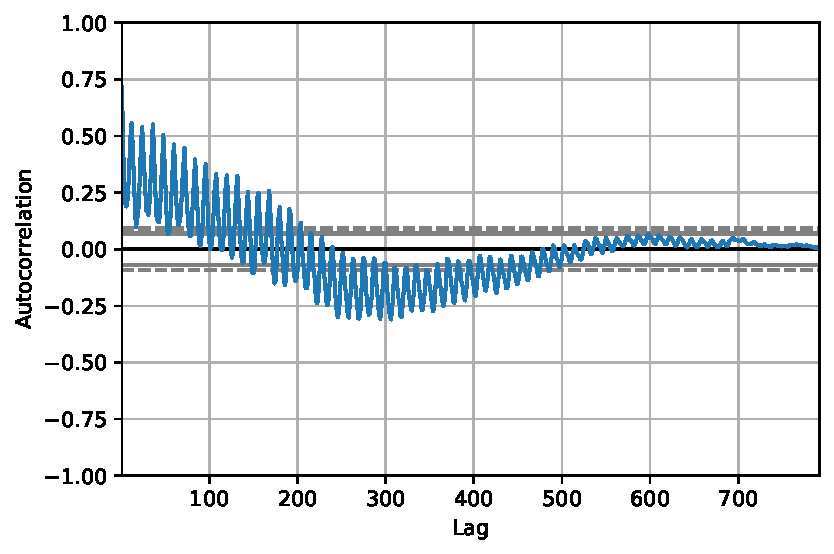
\includegraphics[scale=0.7]{figs/ipc.pdf}
    \caption{Autocorrelation plot for historical inflation.}
    \label{fig:autcorr}
\end{figure}

\end{enumerate}
\bibliographystyle{IEEEtran}
\bibliography{bibs}
\end{document}
